% !TEX root = ./main.tex

\section*{Executive Summary} % (fold)
\label{sec:executive_summary}

Mirror is een bedrijf die in dienst staat van creatievelingen die hun ideeën in drie-dimensionale producten en onderdelen helpt transformeren.

Er wordt gekozen voor een heel dichte samenwerking met high-profile klanten om zich zo op een ander marktsegment te richten dan andere 3D-ontwerpbureaus die vanuit een uitvoerende manier te werk gaan, en enkel luisteren naar de klant, zonder zelf hun expertise te gebruiken om indrukwekkende toepassingen te verkrijgen.

Mirror begint als een eenmanszaak die met een knal zal beginnen door een pop-upwinkel met verwezenlijkte ontwerpen samen te mengen met het artisanale van `Handmade in Brugge'.

% section executive_summary (end)

\section{Missie en visie} % (fold)
\label{sec:missie_en_visie}
\subsection{Golden Circle} % (fold)
\label{ssub:golden_circle}

Voor de visie van Mirror wordt de methode van `Golden Circle'\cite{start-with-why} gebruikt. Deze bepaalt dat het allerbelangrijkste is waarom je je product maakt, daarna pas hoe en als allerlaatste wat je exact maakt, dat is een gevolg van waarom en hoe.

\begin{figure}[H]
  \label{figure:golden-circle}
  \centering
  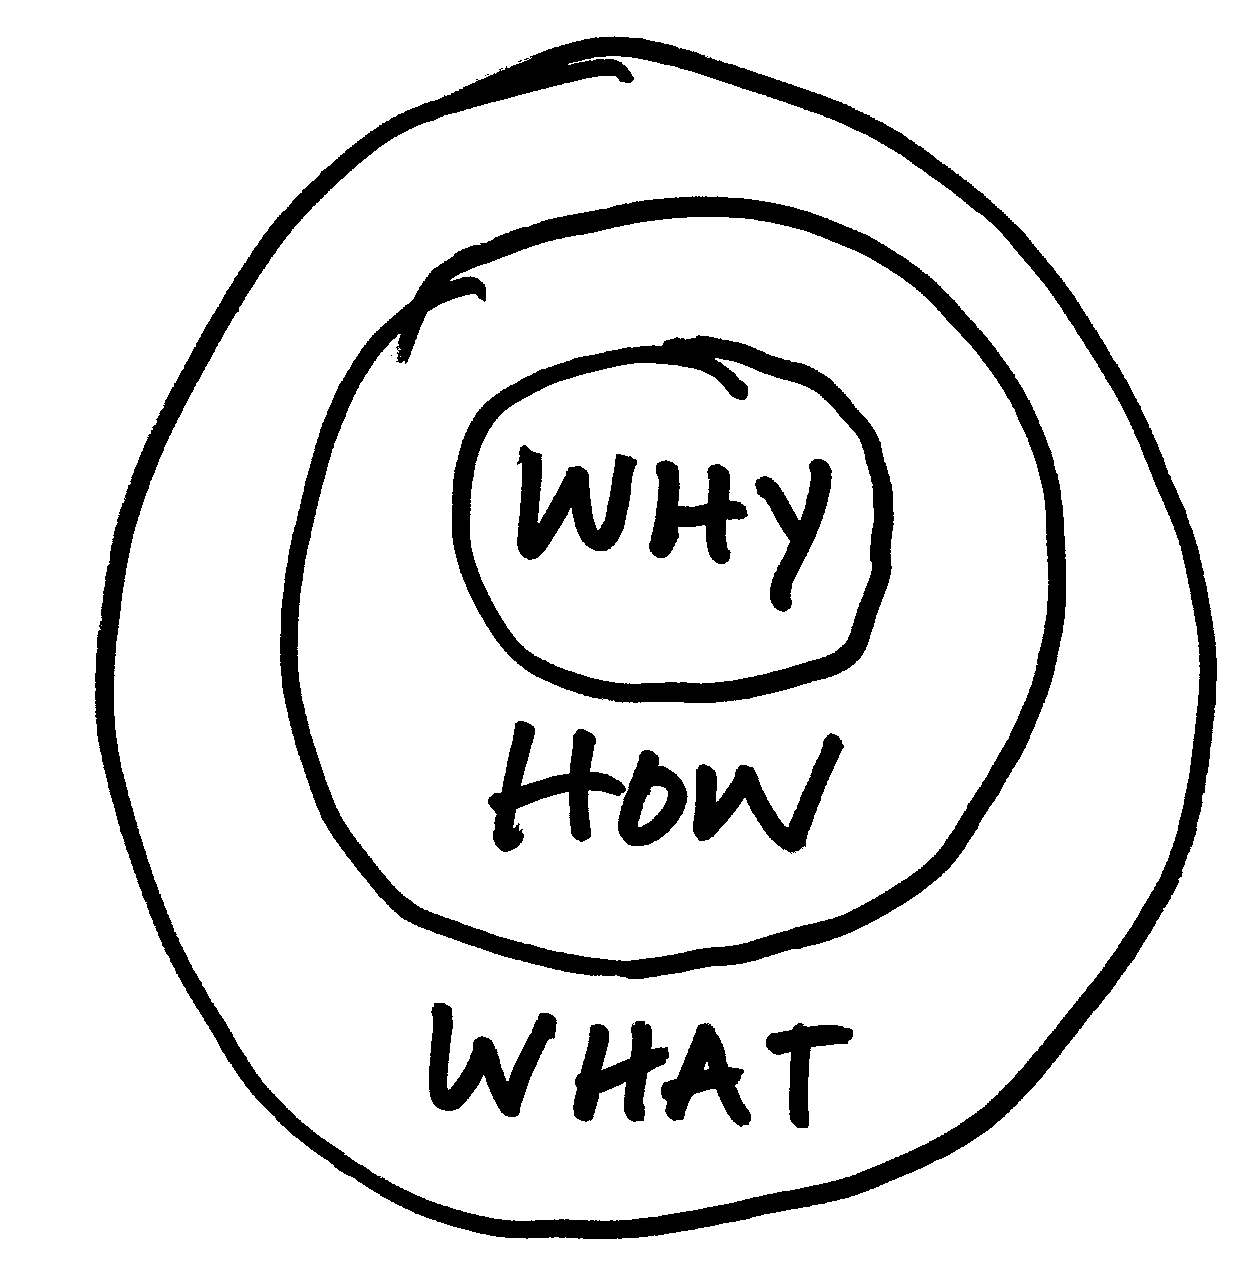
\includegraphics[width=0.5\textwidth]{why-how-what.png}
  \caption{Golden Circle\cite{golden-circle}}
\end{figure}

\paragraph{\textbf{Why} - Waar geloof ik in? Wat is mijn doel?}

innoveren en inspireren
co-creatie
zet de makers in het middelpunt
producten maken om trots op te zijn
link met `Handmade in Brugge'

\paragraph{\textbf{How} - het proces, waarmaken `\textbf{Why}'}

uitwerken ontwerpen en ideeën van makers
klantenbinding
klantnabijheid, verbonden met regio
kwaliteit boven prijs

\paragraph{\textbf{What} – het resultaat, het product}

3D-projecten en lasercutting kwalitatief uitwerken
% subsection golden_circle (end)
\subsection{Missie} % (fold)
\label{sub:missie}
Samen met ontwerpers en makers in de creatieve industrie in de Brugse regio vertalen we ideeën in krachtige 3D-oplossingen.  Mirror is een innovatieve dienstverlener waar de ideeën van de klant in het middelpunt staan.
% subsection missie (end)
\subsection{Visie} % (fold)
\label{sub:visie}
Mirror is een innovatieve dienstverlener in de schaduw van ontwerpers en makers. Heb je als maker een idee in je hoofd of al een gedetailleerd ontwerp? Mirror ondersteunt je in elke fase van het ontwerp tot de uitvoering bij het realiseren van 3D-projecten via 3D-printen, lasercutting\dots Mirror kiest voor een sterke verbondenheid met de regio Brugge en werkt aan een duurzame klantenbinding door co-creatie. Mirror laat jou als maker schitteren.
% subsection visie (end)
\subsection{Naam} % (fold)
\label{sub:naam}

De naam Mirror (spiegel) is gekozen omdat je in een spiegel ziet wat je wil zien, en de werkelijkheid kan combineren met je imaginatie. Mirror gaat verder met dat gevoel en brengt dromen van creatievelingen tot werkelijkheid. Er is heel veel dat je kan doen enkel en alleen met artisanale productiemethodes, de combinatie van het moderne met het traditionele zorgt ervoor dat je het beste kan creëren van beide werelden.

% subsection naam (end)
% section missie_en_visie (end)
